\documentclass[addpoints]{exam}

% Header and footer.
\pagestyle{headandfoot}
\runningheadrule
\runningfootrule
\runningheader{CS 113 Discrete Mathematics}{HW I: Sets}{Spring 2020}
\runningfooter{}{Page \thepage\ of \numpages}{}
\firstpageheader{}{}{}

% \qformat{{\large\bf \thequestion. \thequestiontitle}\hfill[\totalpoints\ points]}
\boxedpoints
\printanswers

\title{Homework I: Sets\\ CS 113 Discrete Mathematics\\ Habib University -- Spring 2020}
\author{sr05848}  % replace with your ID, e.g. oy02945
\date{29-01-2020}
\usepackage{graphicx}

\begin{document}
\maketitle

\begin{questions}


  \question[5]
  Write down $\mathcal{P}(X)$ if 
  $ X = \{ \emptyset, \{\alpha, \beta, \gamma \}, \gamma, \{\{ \alpha, \beta \} \} \}$.
  \begin{solution}
    $\mathcal{P}{X} = \{\emptyset,\{\emptyset\}, \{\alpha,\beta,\gamma\},\{\{\{\alpha,\beta\}\}\},\{\gamma\},\{\emptyset,\{\alpha,\beta,\gamma\}\},\{\emptyset,\gamma\},\{\emptyset,\{\{\alpha,\gamma\}\}\},\{\{\aplha,\beta,\gamma\},\gamma\},\\\{\{\alpha,\beta,\gamma\},\{\{\alpha,\beta\}\}\},\{\gamma,\{\{\alpha,\beta\}\}\},\{\emptyset,\{\alpha,\beta,\gamma\},\gamma\},\{\emptyset,\{\apha,\beta,\gamma\},\{\{\alpha,\beta\}\}\},\{\emptyset,\gamma,\{\{\alpha,\beta\}\}\},\{\{\apha,\beta,\gamma\},\gamma,\{\{\alpha,\beta\}\}\},\\\{\emptyset,\{\alpha,\beta,\gamma\},\gamma,\{\{\alpha,\beta\}\}\}\}$ 
  \end{solution}

  \question
  \begin{parts}
    \part[5] 
    Assume that RO has asked for your help to generate a set that contains all the possible pairs of DSSE faculty and DSSE courses at Habib University. Describe the sets and set operations that you can use to provide RO the desired set.
    \begin{solution}
      $A \times B = \{(x,y)\mid (x \in DSSE \ FACULTY) \ and \ (y \in DSSE \ COURSES)\}$
    \end{solution}

    \part[5] Imagine that the the operation above is extended to include an additional set that contains all the time slots when a course can be scheduled. Explain the outcome of the obtained set.
    \begin{solution}
      $(A \times B) \times C = \{(a,b,c) \mid(a \in FACULTY) \ and \ (b \in COURSES) \ and \ (c \in TIME)$\\ We made a pair of A x B with each element of the time slots in set C.In result each faculty member along with the course are allotted time slots.
    \end{solution}
  \end{parts}
  
  \question
  The \textit{symmetric difference} of two sets $A$ and $B$ is defined as $A\oplus B = (A-B) \cup (B-A)$. It is also known as the \textit{disjunctive union} as it contains all those elements which are in either of those sets, but not in their intersection. 
  \begin{parts}
    \part[5] Prove that $A\oplus B = (A \cup B)-(A \cap B).$
    \begin{solution}
     prove has been done through venn diagram given below, among pair of sets (circles), first one represents A and second one represents B.
    \end{solution}
    \begin{figure}[h!]
        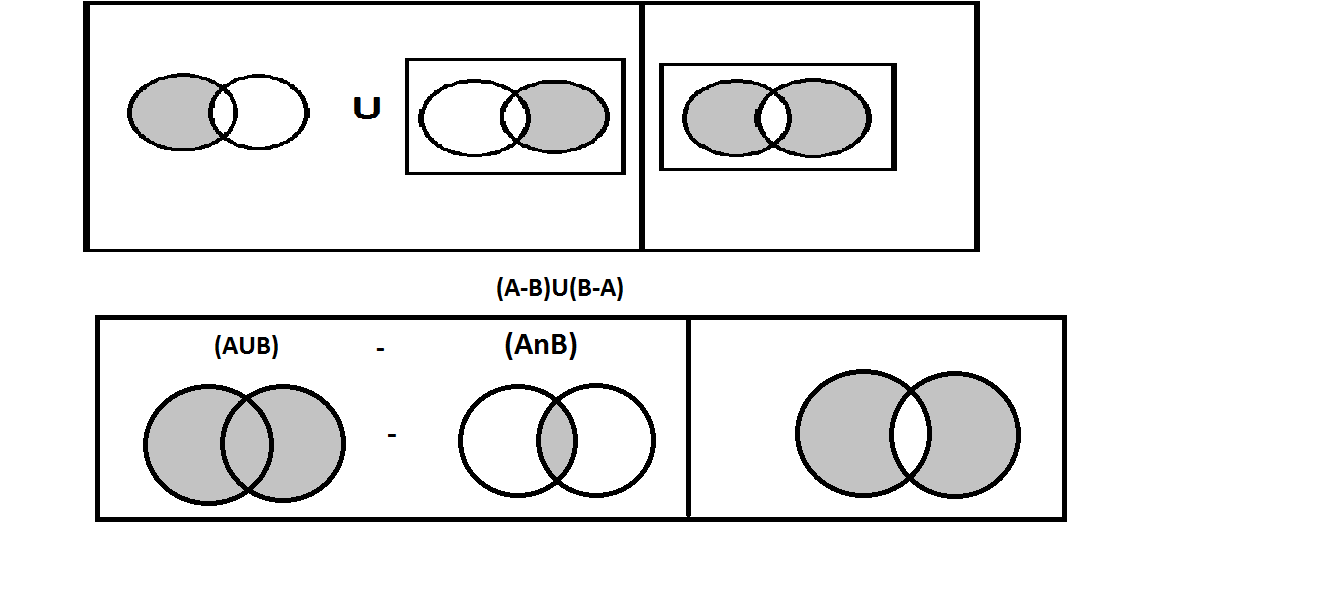
\includegraphics[width=\linewidth]{venn2.png}
                  \caption{diagram}
        \label{fig:venn2}
      \end{figure}
    Figure \ref{fig : venn2.png}

    \part[10] For three sets $A, B,$ and $C$ we definine the symmetric difference as $A\oplus B\oplus C = (A\oplus B)\oplus C $, meaning using the definition twice. Draw the Venn diagram of this set and express it as in part (a).
    \begin{solution}
     Given in part (A): $ A \oplus B =(A \cup B) - (A \cap B) $ \\ With the help of definition, \\ $A \oplus B\oplus C=[ (A \cup B) - (A \cap B) ] \oplus C$ \\ again using the definition, \\ $ A\oplus B\oplus C= [ [(A \cup B) - (A \cap B)] \cup C] - [ [(A \cup B) - (A \cap B)] \cap C] $ 
       
       
    \end{solution}
     \begin{figure}[h!]
        \includegraphics[width=\linewidth]{venn.png}
                  \caption{diagram}
        \label{fig:venn}
      \end{figure}
    Figure \ref{fig : venn.png}
  \end{parts}

  \question
  Let $A$ be the set of all numbers that are divisible by 6 and $B$ the set of all numbers that are divisible by $10$.

  \begin{parts}
    \part[5] Write the sets $A$ and $B$ in proper set notation and describe $A \cap B$ as simply as possible.
    
    \begin{solution}
      $A = \{x \mid x \in \mathbb{R} \land x \%== 6 \}$\\
    $B = \{x \mid x \in \mathbb{R} \land x \% ==10 \}$\\ $ A \cap B  = \{x\mid x \in \mathbb{R} \land x \% = 6 \land x \% == 10 \}$
    \end{solution}
    
    \part[5] What is $A \oplus B$? Describe it using set notation and prove that it is indeed the symmetric difference of $A$ and $B$.
    \begin{solution}
      $A \oplus B=\{\ x \mid x \in A \lor x \in B \land x \notin (A \cap B) \}$ \\
      Where set A is the set of multiples of 6 and set B is the set of multiples of 10.\\
      It is defined as set of those elements which can be the divisible by 6 or can be divisible by 10 but cannot be the disible of both[$ (A \cap B) $] i.e the final set doesn't contain $\{\ 0,30,60... \}$. \\
      If we find $(A-B)$ it will give those elements which are only in A but not in B. For $(B-A) = \{\ 10,20,..)\}$. For $(B-A)$ we will have those elements which are only in B not in A.Hence union of both of these will give $A\oplus B$ 
    \end{solution}

    \part[5] List down the elements of $A$, $B$, and $A \oplus B$ if $U = \{x\in \mathcal{N} \mid x \leq 60 \}$.
    \begin{solution}
      $ A= \{ 0, 6, 12, 18, 24, 30, 36, 42, 48, 54,60 \}$ \\ $ B= \{0, 10, 20, 30, 40, 50, 60 \} $\\ $ A \oplus B = \{6, 10, 12, 18, 20, 24, 36, 40, 42, 48,50, 54 \}$
    \end{solution}
  \end{parts}

  \question
  Show that $\overline{ A \cup \overline{B}} = \overline{A} \cap B$.
  \begin{parts}
    
    \part[5] by using set identities.
    \begin{solution}
       We are using DE MORGAN'S LAW:$ \overline{A}\cap  \overline{B} = \overline{A \cup B}$\\ we have given $\overline{A \cup \overline{B}}$ \\After applying De Morgan's on $\overline {A \cup \overline {B}}$ we'll get $\overline{A} \cap \overline{\overline{B}}$\\ By complementation law: $\overline{A} \cap B$
    \end{solution}
    
    \part[5] by proving that each set is a subset of the other.
    \begin{solution}
      Proving: $ \overline{A \cup \overline {B}} \subseteq \overline {A}\cap B $ \\ $ x \in \overline{A \cup \overline{B}} $ \\ $ x \notin A \cup \overline{B} $ \\ $ x \notin A \lor x \notin \overline{B} $ \\ $ x \in \overline{A} \land x \in B$ \\ $ x \in \overline {A}\cap B $\\\\ Now we will prove that: $ \overline{A} \cap B \subseteq\overline{A \cup \overline{B}}$\\$ x \in \overline{A} \cap B $ \\ $ x \in \overline {A} \land x \in B$ \\ $ x\notin A \lor x\notin B $\\ $ x \notin A \cup \overline {B}$\\ $ x \in \overline {A \cup \overline {B}}$\\Hence,we have proved that each set is a subset of other.
    \end{solution}
  \end{parts}
\end{questions}

\end{document}

